% !TEX root = main.tex
\section{Multiple echo sequences}
\label{sec:Multipleechosequences}
Beside the \textit{Hahn} echo it is also possible to apply multiple \textit{Hahn} echos in one experimental measurement. This method is called \textit{Call-Purcell-Meiboom-Gill}-method (CPMG). Therefore the \SI{180}{\degree} pulse is applied every $2\tau$ and thus there accur many maximums in the signal every $2\tau$. The reason to use the CPMG method is that it is possible to measure the amplitude of two consecutiv maxima more often and therefore the measurement of T$_2$ is more precise. More about this will be discussed in the next chapter.\newline
To make the CPMG signals smoother in the time domain we do not use rectangular functions for the pulses, but smoothen them at the edge by a \textit{sine-bell-square} function. This is possible, due to the fact that it does not change the physical properties of our measurements, but will make them smoother.\newline
A main advantage of CMPG is that errors in the refocusing pulse can be vanished (minimize term of inhomogeneous magnetic field), by changing the phase between the B$_1$ excitation and the refocusing pulses. The program \textit{Prospa} profides a function called ''Constant 180 pulse phase''. This function keeps all the phases of the refocusing pulses equal. The second function \textit{Prospa} provides is ''Alternating 180 pulse phase''. This function compensates echo errors by alternating the refocusing pulses by \SI{180}{\degree}. In figure \ref{fig:180pulsephasedegree} it is visible what a change in the 180 pulse phase does to the signal. Unfortunately we only saved the signal vor 180 pulse phases of \SI{270}{\degree} and \SI{90}{\degree}. For those two values the signal does not change. That is also the reason why there is only one signal visible. The other one is just directly behind the other one and therefore not visible. If we would have saved a pulse phase of \SI{0}{\degree} or \SI{180}{\degree} the signal should change to a way faster decay and so the amplitude dies away really quickly.

\begin{figure}[H]
    \centering
    % GNUPLOT: LaTeX picture with Postscript
\begingroup
  % Encoding inside the plot.  In the header of your document, this encoding
  % should to defined, e.g., by using
  % \usepackage[cp1252,<other encodings>]{inputenc}
  \inputencoding{cp1252}%
  \makeatletter
  \providecommand\color[2][]{%
    \GenericError{(gnuplot) \space\space\space\@spaces}{%
      Package color not loaded in conjunction with
      terminal option `colourtext'%
    }{See the gnuplot documentation for explanation.%
    }{Either use 'blacktext' in gnuplot or load the package
      color.sty in LaTeX.}%
    \renewcommand\color[2][]{}%
  }%
  \providecommand\includegraphics[2][]{%
    \GenericError{(gnuplot) \space\space\space\@spaces}{%
      Package graphicx or graphics not loaded%
    }{See the gnuplot documentation for explanation.%
    }{The gnuplot epslatex terminal needs graphicx.sty or graphics.sty.}%
    \renewcommand\includegraphics[2][]{}%
  }%
  \providecommand\rotatebox[2]{#2}%
  \@ifundefined{ifGPcolor}{%
    \newif\ifGPcolor
    \GPcolorfalse
  }{}%
  \@ifundefined{ifGPblacktext}{%
    \newif\ifGPblacktext
    \GPblacktexttrue
  }{}%
  % define a \g@addto@macro without @ in the name:
  \let\gplgaddtomacro\g@addto@macro
  % define empty templates for all commands taking text:
  \gdef\gplbacktext{}%
  \gdef\gplfronttext{}%
  \makeatother
  \ifGPblacktext
    % no textcolor at all
    \def\colorrgb#1{}%
    \def\colorgray#1{}%
  \else
    % gray or color?
    \ifGPcolor
      \def\colorrgb#1{\color[rgb]{#1}}%
      \def\colorgray#1{\color[gray]{#1}}%
      \expandafter\def\csname LTw\endcsname{\color{white}}%
      \expandafter\def\csname LTb\endcsname{\color{black}}%
      \expandafter\def\csname LTa\endcsname{\color{black}}%
      \expandafter\def\csname LT0\endcsname{\color[rgb]{1,0,0}}%
      \expandafter\def\csname LT1\endcsname{\color[rgb]{0,1,0}}%
      \expandafter\def\csname LT2\endcsname{\color[rgb]{0,0,1}}%
      \expandafter\def\csname LT3\endcsname{\color[rgb]{1,0,1}}%
      \expandafter\def\csname LT4\endcsname{\color[rgb]{0,1,1}}%
      \expandafter\def\csname LT5\endcsname{\color[rgb]{1,1,0}}%
      \expandafter\def\csname LT6\endcsname{\color[rgb]{0,0,0}}%
      \expandafter\def\csname LT7\endcsname{\color[rgb]{1,0.3,0}}%
      \expandafter\def\csname LT8\endcsname{\color[rgb]{0.5,0.5,0.5}}%
    \else
      % gray
      \def\colorrgb#1{\color{black}}%
      \def\colorgray#1{\color[gray]{#1}}%
      \expandafter\def\csname LTw\endcsname{\color{white}}%
      \expandafter\def\csname LTb\endcsname{\color{black}}%
      \expandafter\def\csname LTa\endcsname{\color{black}}%
      \expandafter\def\csname LT0\endcsname{\color{black}}%
      \expandafter\def\csname LT1\endcsname{\color{black}}%
      \expandafter\def\csname LT2\endcsname{\color{black}}%
      \expandafter\def\csname LT3\endcsname{\color{black}}%
      \expandafter\def\csname LT4\endcsname{\color{black}}%
      \expandafter\def\csname LT5\endcsname{\color{black}}%
      \expandafter\def\csname LT6\endcsname{\color{black}}%
      \expandafter\def\csname LT7\endcsname{\color{black}}%
      \expandafter\def\csname LT8\endcsname{\color{black}}%
    \fi
  \fi
    \setlength{\unitlength}{0.0500bp}%
    \ifx\gptboxheight\undefined%
      \newlength{\gptboxheight}%
      \newlength{\gptboxwidth}%
      \newsavebox{\gptboxtext}%
    \fi%
    \setlength{\fboxrule}{0.5pt}%
    \setlength{\fboxsep}{1pt}%
\begin{picture}(7200.00,5040.00)%
    \gplgaddtomacro\gplbacktext{%
      \csname LTb\endcsname%%
      \put(814,704){\makebox(0,0)[r]{\strut{}$-60$}}%
      \put(814,1390){\makebox(0,0)[r]{\strut{}$-40$}}%
      \put(814,2076){\makebox(0,0)[r]{\strut{}$-20$}}%
      \put(814,2762){\makebox(0,0)[r]{\strut{}$0$}}%
      \put(814,3447){\makebox(0,0)[r]{\strut{}$20$}}%
      \put(814,4133){\makebox(0,0)[r]{\strut{}$40$}}%
      \put(814,4819){\makebox(0,0)[r]{\strut{}$60$}}%
      \put(946,484){\makebox(0,0){\strut{}$0$}}%
      \put(1783,484){\makebox(0,0){\strut{}$1000$}}%
      \put(2619,484){\makebox(0,0){\strut{}$2000$}}%
      \put(3456,484){\makebox(0,0){\strut{}$3000$}}%
      \put(4293,484){\makebox(0,0){\strut{}$4000$}}%
      \put(5130,484){\makebox(0,0){\strut{}$5000$}}%
      \put(5966,484){\makebox(0,0){\strut{}$6000$}}%
      \put(6803,484){\makebox(0,0){\strut{}$7000$}}%
    }%
    \gplgaddtomacro\gplfronttext{%
      \csname LTb\endcsname%%
      \put(209,2761){\rotatebox{-270}{\makebox(0,0){\strut{}Amplitude in $\si{\mu \volt}$}}}%
      \put(3874,154){\makebox(0,0){\strut{}Time in $\si{\second}$}}%
      \csname LTb\endcsname%%
      \put(5816,4646){\makebox(0,0)[r]{\strut{}180 pulse phase \SI{270}{\degree}}}%
      \csname LTb\endcsname%%
      \put(5816,4426){\makebox(0,0)[r]{\strut{}180 pulse phase \SI{90}{\degree}}}%
    }%
    \gplbacktext
    \put(0,0){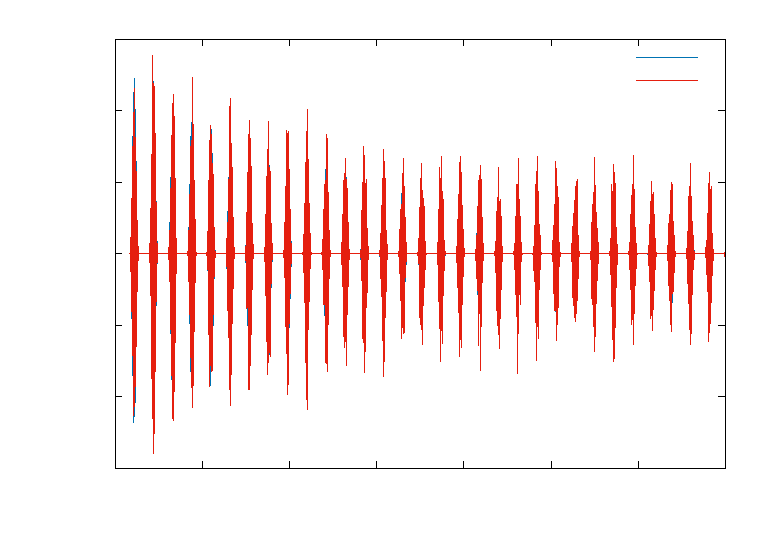
\includegraphics{plots/180pulsephasedegree}}%
    \gplfronttext
  \end{picture}%
\endgroup

    \caption[This figure shows the impact of the 180 pulse phase.]{This figure shows the impact of the 180 pulse phase. Unfortunately we only saved data for a 180 pulse phase of \SI{270}{\degree} and \SI{90}{\degree} and for those values it is correct that the signal does not change, but a signal for a 180 pulse phase of \SI{180}{\degree} would have shown a different signal.}
    \label{fig:180pulsephasedegree}
\end{figure}
